\documentclass[aspectratio=169,10pt]{beamer}

% ============================================================
%  Curso de Maestría — Métodos de Optimización
%  Clase 3: Metaheurísticas
%           (basin hopping, simulated annealing, algoritmos
%            genéticos, particle swarm optimization)
% ============================================================

\usepackage[utf8]{inputenc}
\usepackage[T1]{fontenc}
\usepackage{lmodern}
\usepackage[spanish]{babel}
\usepackage{amsmath,amssymb,amsthm}
\usepackage{graphicx}
\usepackage{booktabs}
\usepackage{xcolor}
\usepackage{listings}
\usepackage{tikz}

\graphicspath{{figs/}}

\usetheme{metropolis}
\metroset{block=fill, progressbar=frametitle, sectionpage=progressbar, numbering=fraction}

\definecolor{pygreen}{RGB}{0,128,0}
\definecolor{pyblue}{RGB}{0,0,180}
\definecolor{pygray}{RGB}{110,110,110}
\definecolor{codebg}{RGB}{245,245,245}

\lstdefinestyle{pythonstyle}{
  language=Python,
  backgroundcolor=\color{codebg},
  basicstyle=\ttfamily\scriptsize,
  keywordstyle=\color{pyblue}\bfseries,
  commentstyle=\color{pygreen}\itshape,
  stringstyle=\color{pygray},
  numbers=none,
  breaklines=true,
  showstringspaces=false,
  frame=single,
  rulecolor=\color{gray!40},
  xleftmargin=4pt,
  xrightmargin=4pt,
  aboveskip=6pt,
  belowskip=2pt,
}
\lstset{style=pythonstyle}

% --- notación abreviada ---
\newcommand{\R}{\mathbb{R}}
\newcommand{\grad}{\nabla}
\newcommand{\x}{\mathbf{x}}

\title{Métodos de Optimización}
\subtitle{Clase 3: Metaheurísticas}
\author{[Nombre del profesor]}
\institute{Programa de Maestría, [Nombre de la universidad / programa]}
\date{Septiembre de 2026}

\begin{document}

% ---------------------------------------------------------------
\begin{frame}[plain]
  \maketitle
\end{frame}

\begin{frame}{Contenido}
  \footnotesize
  \begin{columns}[T]
    \column{0.5\textwidth}
    \begin{enumerate}
      \setcounter{enumi}{0}
      \item Motivación: de random walk a las metaheurísticas
      \item Basin hopping
      \item El criterio de Metrópolis y la temperatura $T$
      \item La magnitud del salto: \texttt{step\_size}
      \item Simulated annealing
    \end{enumerate}
    \column{0.5\textwidth}
    \begin{enumerate}
      \setcounter{enumi}{5}
      \item Algoritmos genéticos
      \item Particle swarm optimization
      \item Síntesis: 9 métodos, un solo paisaje
      \item Roadmap del curso
      \item Ejercicios y referencias
    \end{enumerate}
  \end{columns}
\end{frame}

% ==================================================================
\section{Motivación}
% ==================================================================

\begin{frame}{De la Clase 2 a las metaheurísticas}
  \begin{block}{Lo que vimos en la Clase 2}
    Bisección y áurea (1D), grid search ($O(N^d)$), random walk y
    Nelder--Mead. Todos son \textbf{locales} o de \textbf{costo
    exponencial}: ninguno tiene una estrategia inteligente para escapar
    de un mínimo local malo.
  \end{block}
  \begin{alertblock}{La pregunta que quedó abierta}
    ¿Cómo combinar la \textbf{eficiencia} de un optimizador local (como
    Nelder--Mead o el descenso de gradiente) con la \textbf{capacidad de
    escapar} de mínimos locales (como random walk, pero de forma más
    inteligente)?
  \end{alertblock}
  Hoy: cuatro respuestas a esa pregunta, cada una con una idea distinta
  de cómo \emph{inyectar aleatoriedad útil} en la búsqueda.
\end{frame}

\begin{frame}{El paisaje de siempre}
  Seguimos con la misma función de 6 pozos de la Clase 2
  (\texttt{scripts/\_landscape.py}), donde ya vimos que random walk
  greedy se queda atrapado en $f=-0.54$ y hasta Powell (scipy) converge
  al falso mínimo $(0,0)$ con $f\approx0$. El mínimo global real está en
  $x^*\approx(-6.37,\,3.92)$, $f^*\approx-3.29$.
  \begin{block}{Idea unificadora: random walk como caso límite}
    \begin{itemize}
      \item Random walk \textbf{greedy} $\;=\;$ aceptar un salto peor con
        probabilidad $0$ (nunca).
      \item Random walk \textbf{puro} $\;=\;$ aceptar un salto peor con
        probabilidad $1$ (siempre).
    \end{itemize}
    Las metaheurísticas de hoy generalizan esto: aceptan un salto peor
    con una probabilidad \textbf{intermedia}, controlada por un
    parámetro de \emph{temperatura} $T$.
  \end{block}
\end{frame}

% ==================================================================
\section{Basin hopping}
% ==================================================================

\begin{frame}{Basin hopping: la idea (Wales \& Doye, 1997)}
  \begin{block}{Algoritmo}
    \begin{enumerate}
      \item Partir de $\x_{\text{cur}}$, un mínimo local (via descenso de
        gradiente u otro optimizador local).
      \item Perturbar: $\x_{\text{prop}} = \x_{\text{cur}} + \Delta$, con
        $\Delta$ un salto aleatorio de magnitud \texttt{step\_size}.
      \item \textbf{Reoptimizar localmente} desde $\x_{\text{prop}}$
        $\to$ nuevo mínimo local $\x_{\text{new}}$, $f_{\text{new}}$.
      \item \textbf{Aceptar} con el criterio de Metrópolis (siguiente
        sección): siempre si $f_{\text{new}}<f_{\text{cur}}$; si no, con
        probabilidad $e^{-\Delta E/T}$.
      \item Guardar aparte el mejor $(\x_{\text{best}}, f_{\text{best}})$
        visto en \textbf{toda} la corrida (no solo el actual).
    \end{enumerate}
  \end{block}
  \begin{alertblock}{La clave}
    Cada salto aterriza \textbf{en el fondo de una cuenca} (no en
    cualquier punto) porque siempre se reoptimiza — así \emph{saltamos entre
    mínimos locales} en vez de caminar sin rumbo como random walk.
  \end{alertblock}
\end{frame}

\begin{frame}[fragile]{Basin hopping: código manual (núcleo)}
\begin{lstlisting}
def local_search(x0, lr=0.1, max_iter=2000, tol=1e-8):
    x = np.array(x0, dtype=float)
    for _ in range(max_iter):
        g = grad_f(*x)                    # gradiente numerico
        if np.linalg.norm(g) < tol: break
        x = x - lr*g                      # paso FIJO y chico:
    return x, float(f(*x))                # evita "saltar" de cuenca

def basin_hopping_manual(x0, n_iter=40, step_size=7.0, T=1.5, seed=0):
    rng = np.random.default_rng(seed)
    x_cur, f_cur = local_search(x0)
    x_best, f_best = x_cur.copy(), f_cur
    for it in range(n_iter):
        x_prop = x_cur + rng.uniform(-step_size, step_size, size=2)
        x_new, f_new = local_search(x_prop)
        aceptado = (f_new < f_cur) or \
                   (rng.random() < np.exp(-(f_new - f_cur)/T))
        if aceptado: x_cur, f_cur = x_new, f_new
        if f_new < f_best: x_best, f_best = x_new.copy(), f_new
    return x_best, f_best
\end{lstlisting}
\end{frame}

\begin{frame}[fragile]{Basin hopping: ejemplo paso a paso}
  Arrancando en $x_0=(8,-8)$, \texttt{step\_size=7.0}, $T=1.5$:
  \tiny
\begin{lstlisting}
it= 1  x_new=[ 4.85 -4.85]  f_new=-0.5442  f_cur=-0.5442  -> ACEPTADO
it= 2  x_new=[-0.  -0.  ]  f_new=-0.0000  f_cur=-0.5442  -> rechazado
it= 4  x_new=[4.91  3.93]  f_new=-2.7920  f_cur=-0.5442  -> ACEPTADO
it= 6  x_new=[0.    5.80]  f_new=-0.7552  f_cur=-2.7920  -> ACEPTADO (peor, sorteo!)
it= 9  x_new=[-6.37  3.92]  f_new=-3.2880  f_cur=-0.0000  -> ACEPTADO
      ...
it=40  ->  x* = [-6.3698, 3.9191]   f(x*) = -3.2880   (el GLOBAL)
\end{lstlisting}
  \normalsize
  En la iteración 6 se acepta un punto \textbf{peor} que el actual — eso
  es lo que permite, más adelante, escapar hacia el pozo global en la
  iteración 9. Sin ese \emph{sorteo} el algoritmo se habría quedado en
  $(4.91,3.93)$, $f=-2.79$.
\end{frame}

\begin{frame}{Basin hopping: trayectoria completa}
  \begin{center}
    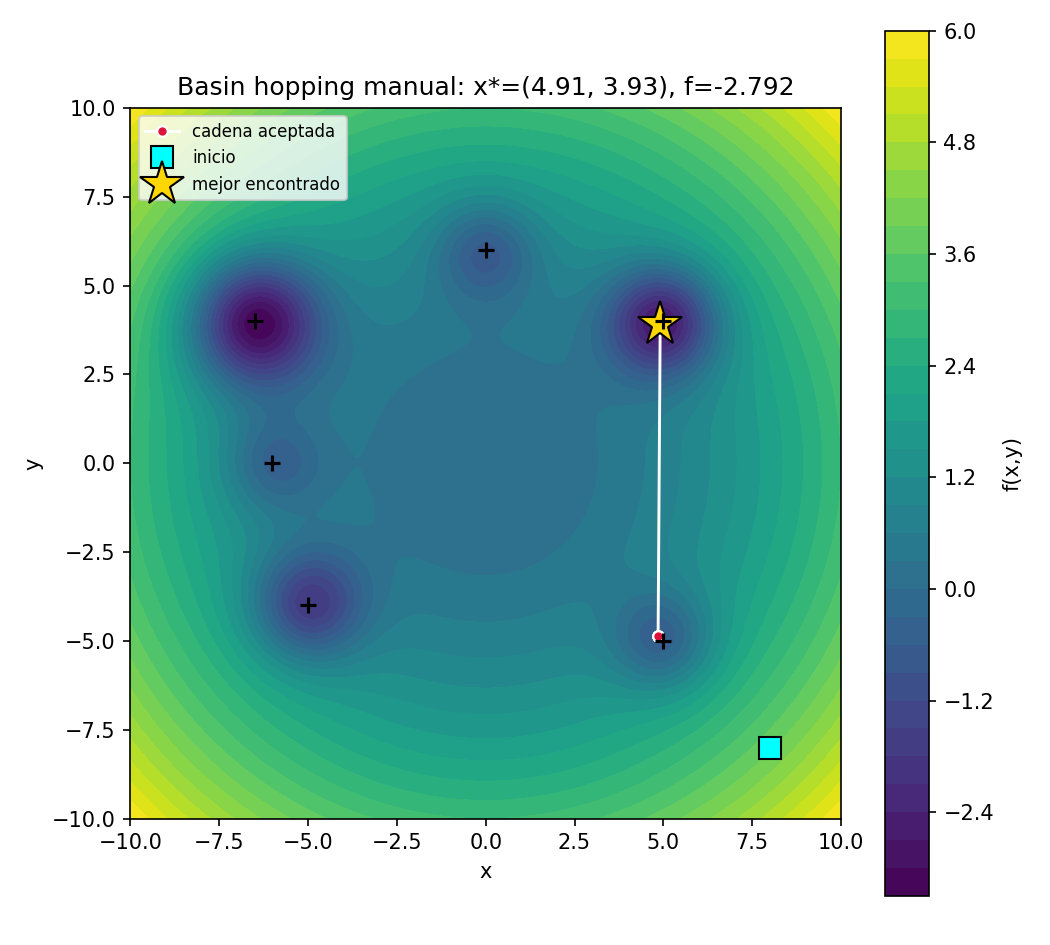
\includegraphics[height=6.2cm,keepaspectratio]{fig01_basin_hopping.png}
  \end{center}
\end{frame}

\begin{frame}[fragile]{Basin hopping: manual vs.\ scipy}
  \begin{columns}
    \column{0.55\textwidth}
    \textbf{Con scipy (mismos parámetros):}
\begin{lstlisting}
from scipy.optimize import basinhopping

res = basinhopping(
    lambda p: f(p[0], p[1]), x0,
    niter=40,
    minimizer_kwargs={"method": "BFGS"},
    stepsize=7.0, T=1.5, seed=0)
\end{lstlisting}
    \column{0.45\textwidth}
    \small Manual: $x^*=(-6.37,3.92)$, $f^*=-3.288$
    (\textbf{el global}). \\[4pt]
    Scipy: $x^*=(4.91,3.93)$, $f^*=-2.792$ (un
    local, \textbf{no} el global).
  \end{columns}
  \begin{alertblock}{Lección: metaheurística $\ne$ garantía}
    Ambas implementaciones son razonables; la diferencia viene de la
    \textbf{secuencia de aleatoriedad} y del optimizador local usado
    (gradiente fijo vs.\ BFGS). Basin hopping mejora las probabilidades
    de encontrar el global, \textbf{no las garantiza} en una sola corrida.
    Con más iteraciones, ambas convergerían con alta probabilidad.
  \end{alertblock}
  Script completo: \texttt{scripts/01\_basin\_hopping.py}
\end{frame}

% ==================================================================
\section{Metrópolis y temperatura}
% ==================================================================

\begin{frame}{El criterio de Metrópolis}
  \begin{block}{Regla de aceptación}
    Sea $\Delta E = f_{\text{new}} - f_{\text{cur}}$ (positivo si el
    salto \emph{empeora}).
    \[
      P(\text{aceptar}) =
      \begin{cases}
        1 & \text{si } \Delta E \le 0 \text{ (mejora o queda igual)} \\
        e^{-\Delta E / T} & \text{si } \Delta E > 0 \text{ (empeora)}
      \end{cases}
    \]
  \end{block}
  \begin{itemize}
    \item $T\to 0$: $e^{-\Delta E/T}\to 0$ para cualquier $\Delta E>0$
      $\;\Rightarrow\;$ \textbf{nunca} acepta empeorar $=$ random walk
      \emph{greedy}.
    \item $T\to\infty$: $e^{-\Delta E/T}\to 1$ $\;\Rightarrow\;$
      \textbf{siempre} acepta $=$ random walk \emph{puro}.
    \item $T$ intermedio: acepta empeorar \textbf{a veces}, más seguido
      si $\Delta E$ es chico (un empeoramiento leve) que si es grande.
  \end{itemize}
\end{frame}

\begin{frame}{Curvas $P(\text{aceptar})$ vs.\ $\Delta E$, por temperatura}
  \begin{center}
    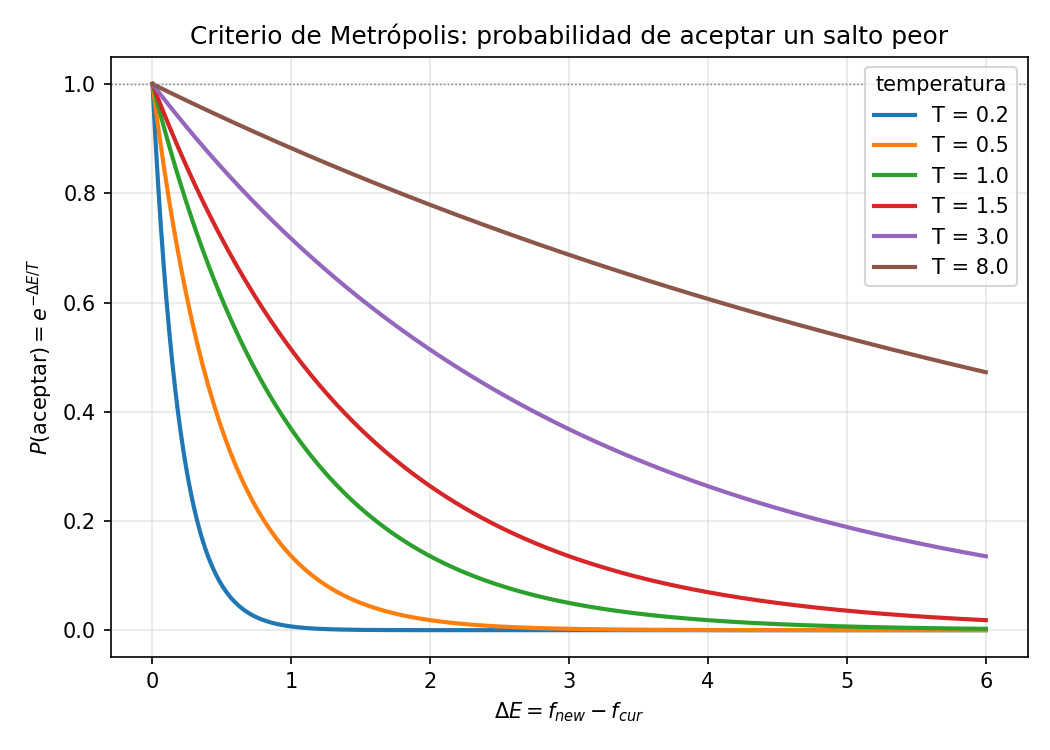
\includegraphics[height=6.4cm,keepaspectratio]{fig02_metropolis_curvas_T.png}
  \end{center}
\end{frame}

\begin{frame}[fragile]{El sorteo: cómo se implementa una probabilidad}
  \begin{block}{La idea}
    Para aceptar con probabilidad $P\in[0,1]$: sortear
    $u\sim\mathcal U(0,1)$ y aceptar si $u<P$. Como $u$ es uniforme,
    $\Pr(u<P)=P$ exactamente.
  \end{block}
\begin{lstlisting}
aceptado = (f_new < f_cur) or (rng.random() < np.exp(-dE/T))
\end{lstlisting}
  \textbf{Verificación empírica} (100{,}000 sorteos por caso):
  \tiny
\begin{lstlisting}
 DeltaE     T   P teorica   tasa observada
   1.00  0.50      0.1353           0.1376
   2.50  1.50      0.1889           0.1885
   0.30  1.00      0.7408           0.7405
   4.00  2.00      0.1353           0.1352
\end{lstlisting}
  \normalsize
  La tasa observada coincide con $P$ hasta el tercer decimal: el sorteo
  hace exactamente lo que promete. Script: \texttt{scripts/02\_metropolis\_y\_temperatura.py}
\end{frame}

% ==================================================================
\section{Magnitud del salto: step\_size}
% ==================================================================

\begin{frame}{¿Qué tan grande debe ser el salto aleatorio?}
  \begin{block}{El compromiso}
    \begin{itemize}
      \item \textbf{step\_size muy chico}: el salto casi nunca saca al
        punto de la cuenca actual $\Rightarrow$ \texttt{local\_search}
        vuelve casi siempre al mismo mínimo $\Rightarrow$ se queda
        atascado (basin hopping degenera a optimización local pura).
      \item \textbf{step\_size muy grande}: el salto cae en zonas
        \emph{lejanas y casi al azar} del paisaje $\Rightarrow$ se pierde
        la ventaja de \emph{caminar entre cuencas vecinas} y el método
        degenera a \textbf{random restart} puro (equivalente a probar
        puntos iniciales al azar, sin aprovechar la estructura local).
      \item \textbf{step\_size razonable}: comparable a la
        \textbf{distancia típica entre mínimos locales} del paisaje.
    \end{itemize}
  \end{block}
\end{frame}

\begin{frame}{Efecto del \texttt{step\_size}: experimento}
  \begin{center}
    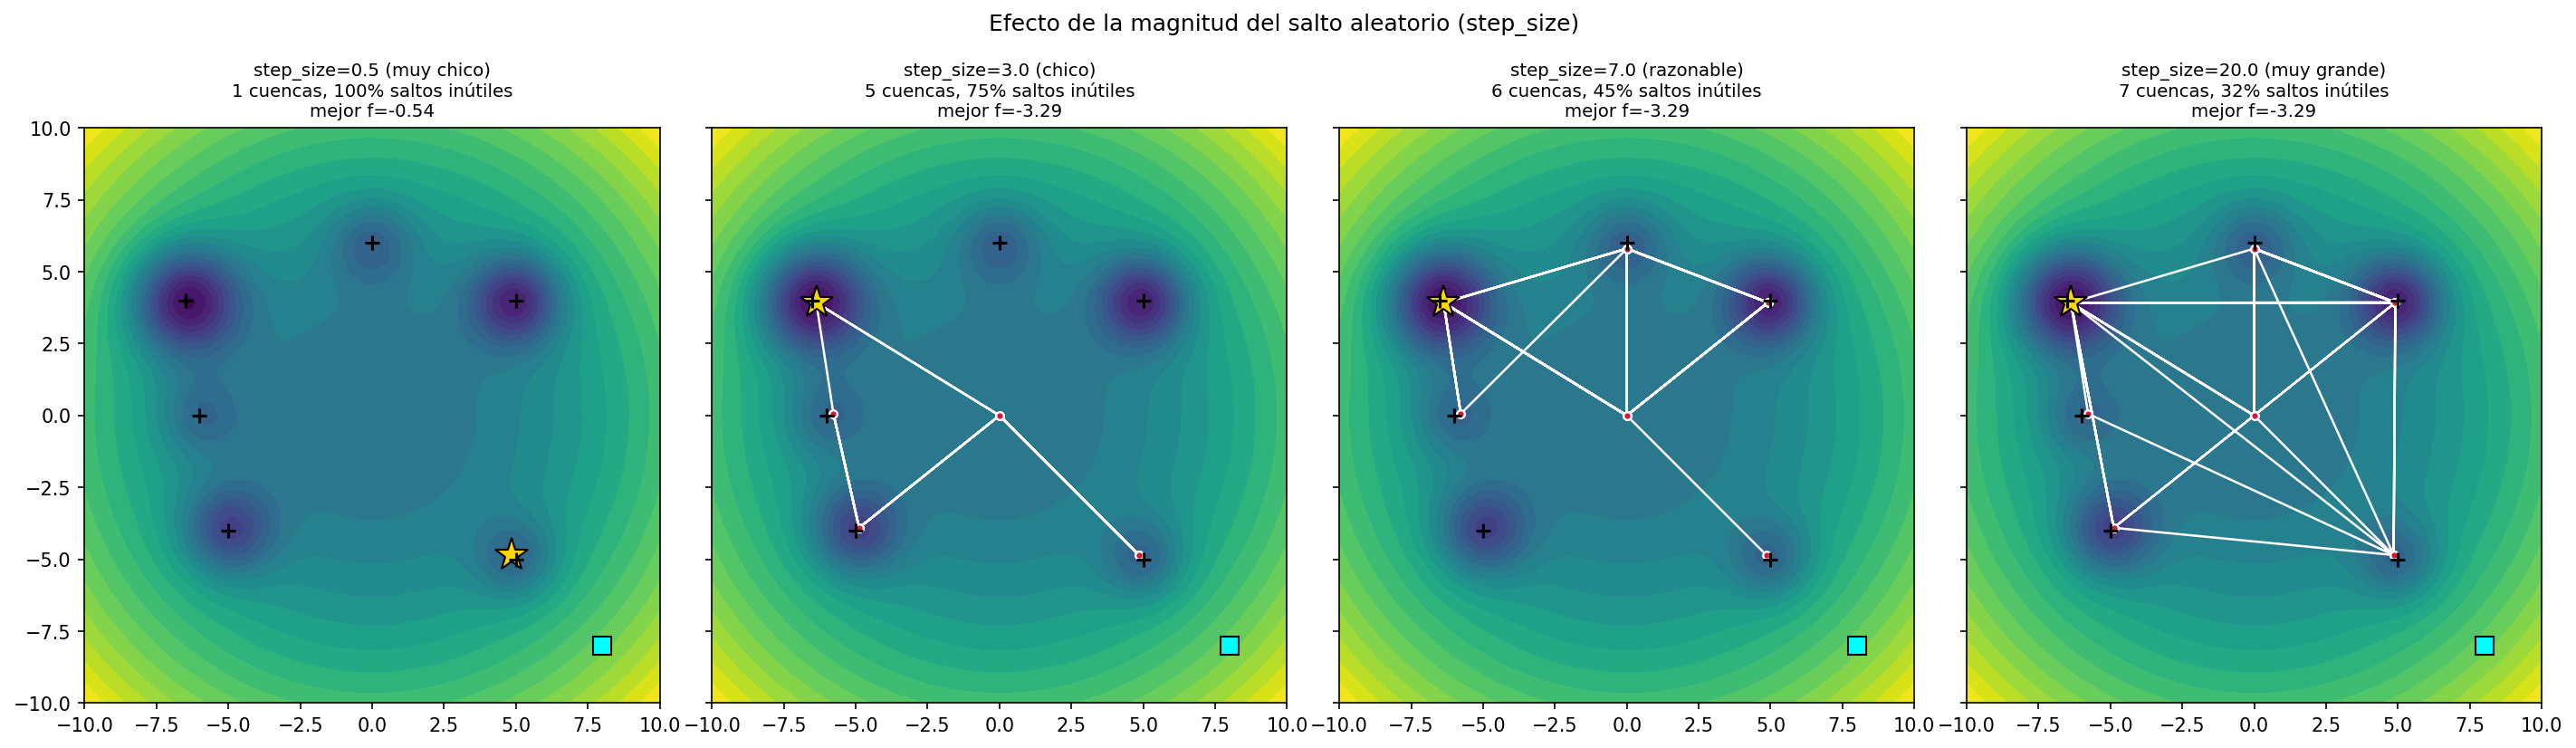
\includegraphics[width=0.95\textwidth,height=5.3cm,keepaspectratio]{fig03_step_size.png}
  \end{center}
  \footnotesize \texttt{step\_size=0.5}: 100\% de los saltos son
  \emph{inútiles} (vuelven a la misma cuenca), 1 sola cuenca visitada, no
  encuentra el global. \texttt{step\_size=7.0} (comparable a la
  separación entre pozos, $\sim 9$--$13$ unidades): mejor balance,
  visita 6 cuencas y encuentra el global. Script:
  \texttt{scripts/03\_step\_size\_efecto.py}
\end{frame}

% ==================================================================
\section{Simulated annealing}
% ==================================================================

\begin{frame}{Simulated annealing: la idea (Kirkpatrick et al., 1983)}
  \begin{alertblock}{Diferencia clave con basin hopping}
    Basin hopping perturba y \textbf{siempre reoptimiza localmente}
    antes de comparar. Simulated annealing perturba el punto actual y
    \textbf{compara/acepta directamente} con Metrópolis, \textbf{sin}
    minimizar en cada paso. El \emph{aterrizaje} en un mínimo ocurre solo al
    final, cuando $T$ ya es chica.
  \end{alertblock}
  \begin{block}{Esquema de enfriamiento (templado)}
    $T$ empieza alta (explora como random walk puro) y decrece con las
    iteraciones (converge como random walk greedy). El más simple y
    usado es el \textbf{geométrico}:
    \[
      T_k = T_0 \, \alpha^k , \qquad 0<\alpha<1 \ \text{(t\'{\i}picamente
      } 0.90\text{--}0.99\text{)}
    \]
  \end{block}
  Así, simulated annealing es literalmente el \emph{puente} entre random walk
  greedy y puro que anticipamos en la Clase 2, con $T$ variando en el
  tiempo en vez de fija.
\end{frame}

\begin{frame}[fragile]{Simulated annealing: código manual}
\begin{lstlisting}
def simulated_annealing_manual(x0, T0=8.0, alpha=0.96, n_iter=200,
                                paso=1.5, seed=0):
    rng = np.random.default_rng(seed)
    x_cur = np.array(x0, dtype=float);  f_cur = float(f(*x_cur))
    x_best, f_best = x_cur.copy(), f_cur
    T = T0
    for it in range(n_iter):
        x_prop = x_cur + rng.normal(scale=paso, size=2)   # SIN reoptimizar
        f_prop = float(f(*x_prop))
        dE = f_prop - f_cur
        aceptado = dE < 0 or rng.random() < np.exp(-dE / T)
        if aceptado: x_cur, f_cur = x_prop, f_prop
        if f_cur < f_best: x_best, f_best = x_cur.copy(), f_cur
        T *= alpha                                         # enfriar
    return x_best, f_best
\end{lstlisting}
\end{frame}

\begin{frame}{Simulated annealing: trayectoria y enfriamiento}
  \begin{center}
    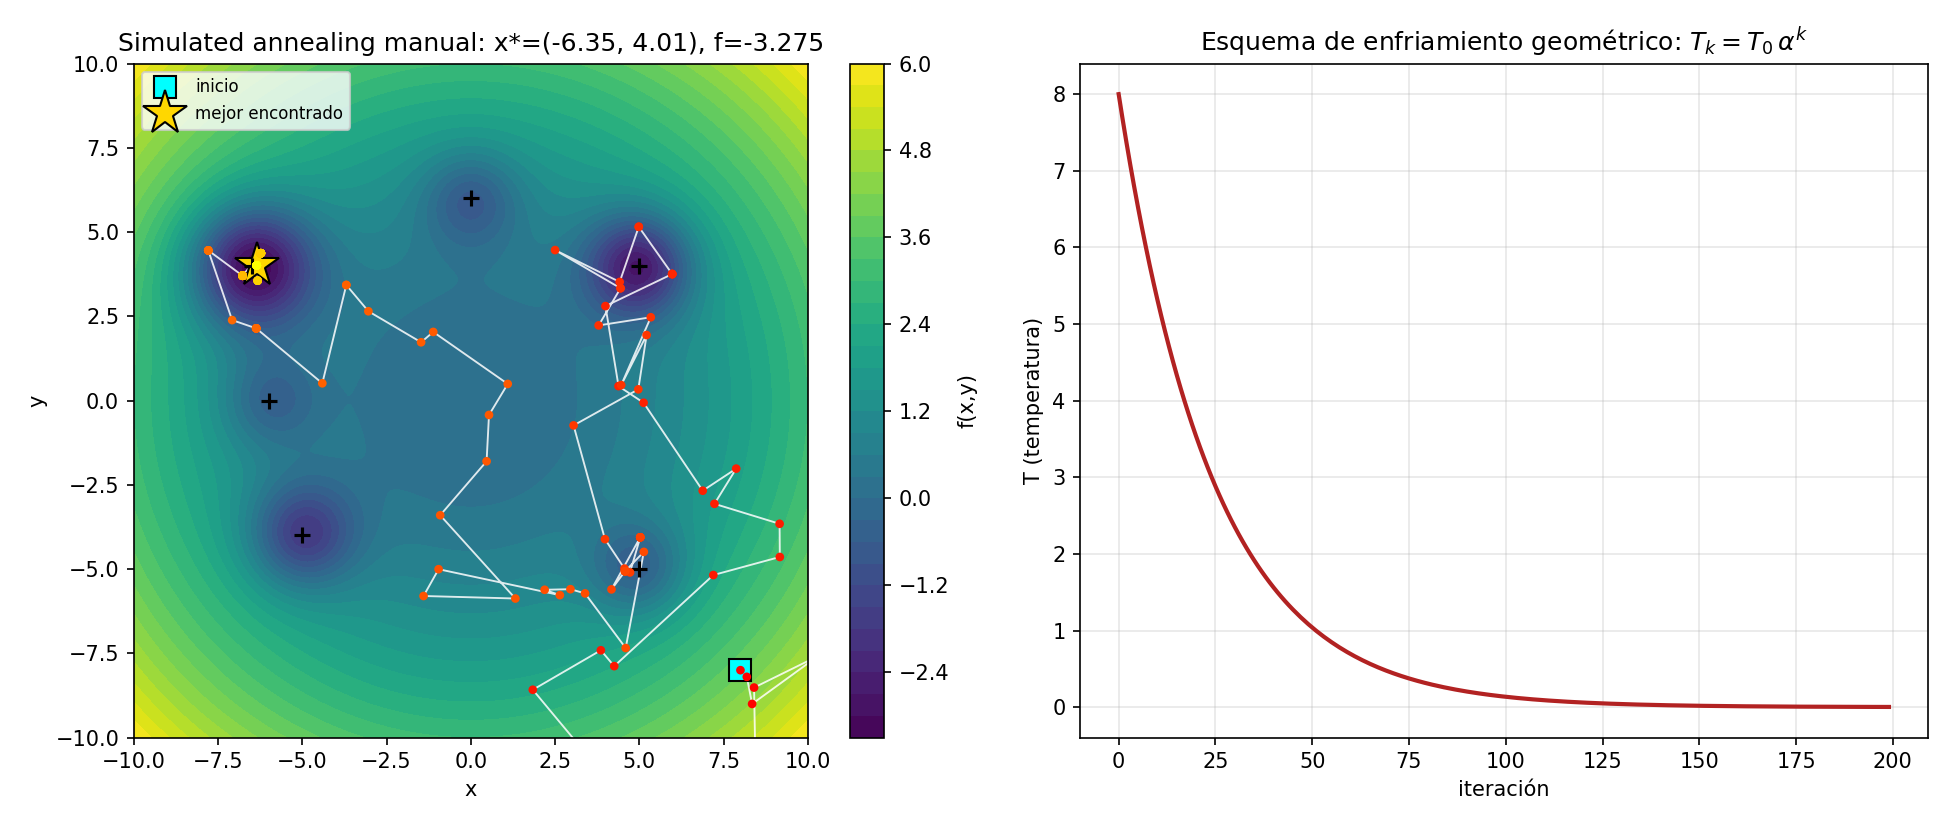
\includegraphics[width=0.92\textwidth,height=4.6cm,keepaspectratio]{fig04_simulated_annealing.png}
  \end{center}
  \footnotesize Izquierda: la cadena difunde ampliamente al inicio ($T$
  alta) y se estabiliza cerca del mejor pozo al final ($T\approx0$).
  Derecha: enfriamiento geométrico $T_k=T_0\alpha^k$. Manual:
  $f^*=-3.275$; \texttt{scipy.optimize.dual\_annealing}: $f^*=-3.288$
  (esquema de enfriamiento y reinicios más sofisticados). Script:
  \texttt{scripts/04\_simulated\_annealing.py}
\end{frame}

% ==================================================================
\section{Algoritmos genéticos}
% ==================================================================

\begin{frame}{Algoritmos genéticos: la idea (Holland, 1975)}
  \begin{block}{De un punto a una \textbf{población}}
    En vez de mover un solo punto, mantenemos $N$ soluciones candidatas
    a la vez y las hacemos \emph{evolucionar}:
    \begin{enumerate}
      \item \textbf{Fitness}: qué tan buena es cada solución ($-f$, si
        minimizamos).
      \item \textbf{Selección}: los mejores individuos tienen más
        chance de \emph{reproducirse} (aquí: torneo — se sortean $k$
        individuos y gana el mejor).
      \item \textbf{Cruce (crossover)}: combinar dos padres para crear un
        hijo. Con valores reales, cruce \textbf{aritmético}:
        $\text{hijo}=\beta\,p_1+(1-\beta)\,p_2$, $\beta\sim U(0,1)$.
      \item \textbf{Mutación}: perturbación aleatoria chica, con
        probabilidad $p_{\text{mut}}$, para mantener diversidad.
      \item \textbf{Elitismo}: los mejores individuos pasan sin cambios
        a la siguiente generación (no se pierde lo mejor logrado).
    \end{enumerate}
  \end{block}
\end{frame}

\begin{frame}[fragile]{Algoritmos genéticos: código manual (núcleo)}
\begin{lstlisting}
def algoritmo_genetico(n_pob=30, n_gen=60, k_torneo=3, p_mut=0.25,
                        sigma_mut=1.0, n_elite=2, seed=0):
    pob = poblacion_inicial(n_pob, rng)         # N puntos al azar
    fit = -f(pob[:,0], pob[:,1])
    for gen in range(n_gen):
        orden = np.argsort(-fit);  pob, fit = pob[orden], fit[orden]
        nueva_pob = [pob[i].copy() for i in range(n_elite)]  # elitismo
        while len(nueva_pob) < n_pob:
            p1 = seleccion_torneo(pob, fit, k_torneo, rng)
            p2 = seleccion_torneo(pob, fit, k_torneo, rng)
            hijo = cruce_aritmetico(p1, p2, rng)
            hijo = mutar(hijo, p_mut, sigma_mut, rng)
            nueva_pob.append(hijo)
        pob = np.array(nueva_pob);  fit = -f(pob[:,0], pob[:,1])
\end{lstlisting}
  \small La \textbf{diversidad de la población} juega el papel que en
  basin hopping/SA jugaba el salto aleatorio: varios individuos exploran
  distintas cuencas \textbf{en paralelo}.
\end{frame}

\begin{frame}{Selección por torneo: la idea, sin código}
  \begin{block}{Dos pasos, nada más}
    \begin{enumerate}
      \item \textbf{Sorteo}: de \emph{toda} la población (los $N$
        individuos completos, no un subconjunto ya filtrado), se sacan
        $k$ al azar, con la misma probabilidad para todos sin importar
        su fitness.
      \item \textbf{Torneo}: de esos $k$ sorteados, gana el de mejor
        fitness. Sin más azar -- es una comparación directa.
    \end{enumerate}
  \end{block}
  \begin{alertblock}{Un error común}
    Torneo \textbf{no} empieza escogiendo de antemano ``los mejores'' y
    sorteando ahí adentro -- eso sería \emph{truncamiento}, donde los
    débiles quedan eliminados de raíz. En torneo el sorteo siempre parte
    de la población completa; el filtro hacia lo bueno ocurre
    indirectamente, sorteo tras sorteo, no de una vez.
  \end{alertblock}
  El tamaño $k$ del sorteo controla la presión selectiva: $k$ grande
  $\Rightarrow$ casi siempre gana el mejor de todos (muy elitista, poca
  diversidad); $k$ chico $\Rightarrow$ más fácil que gane alguien
  mediocre por competir solo contra peores (más diversidad).
\end{frame}

\begin{frame}{Dos padres, dos sorteos -- y la élite también compite}
  \begin{itemize}
    \item Cada hijo necesita dos padres ($p_1$, $p_2$): son
      \textbf{dos sorteos independientes}, cada uno con su propio
      grupo de $k$ individuos extraído de la población completa. Como
      cada sorteo vuelve a empezar de cero, $p_1$ y $p_2$ pueden
      terminar siendo el mismo individuo -- no hay ninguna regla que lo
      impida.
    \item El \textbf{elitismo} (los $n_{\text{elite}}$ mejores pasan
      intactos a la siguiente generación) y la \textbf{selección por
      torneo} son dos mecanismos distintos que conviven: la élite
      \textbf{no se excluye} del sorteo -- sigue en la población y,
      gracias a su buen fitness, tiene muy buenas chances de además
      ganar un torneo y convertirse en padre.
    \item La diferencia real entre ser élite o no: la élite tiene
      \emph{asegurada} una copia en la siguiente generación sin pasar
      por el sorteo; el resto solo puede influir en la siguiente
      generación si gana un torneo.
  \end{itemize}
\end{frame}

\begin{frame}[fragile]{Cruce aritmético: ¿por qué $\beta$ es aleatorio?}
\begin{lstlisting}
def cruce_aritmetico(p1, p2, rng):
    beta = rng.random()          # beta ~ U(0,1), nuevo en CADA cruce
    return beta * p1 + (1 - beta) * p2
\end{lstlisting}
  $\beta$ decide en qué punto del segmento que une a los padres cae el
  hijo: $\beta$ cercano a 1 $\to$ hijo casi igual a $p_1$; cercano a 0
  $\to$ casi igual a $p_2$; $\beta=0.5$ $\to$ exactamente el punto
  medio.
  \begin{alertblock}{¿Por qué no fijar $\beta=0.5$ siempre?}
    Si todo hijo fuera siempre el promedio exacto de sus padres, la
    población tendería a colapsar hacia el centro del espacio de
    búsqueda muy rápido, perdiendo diversidad. Sortear $\beta$ en cada
    cruce hace que unos hijos se parezcan más a un padre y otros al
    otro, conservando variedad.
  \end{alertblock}
  Nota: aquí se sortea un único $\beta$ por cruce (mismo valor para $x$
  e $y$); existe una variante con un $\beta$ distinto por coordenada.
\end{frame}

\begin{frame}{Algoritmos genéticos: población final y convergencia}
  \begin{center}
    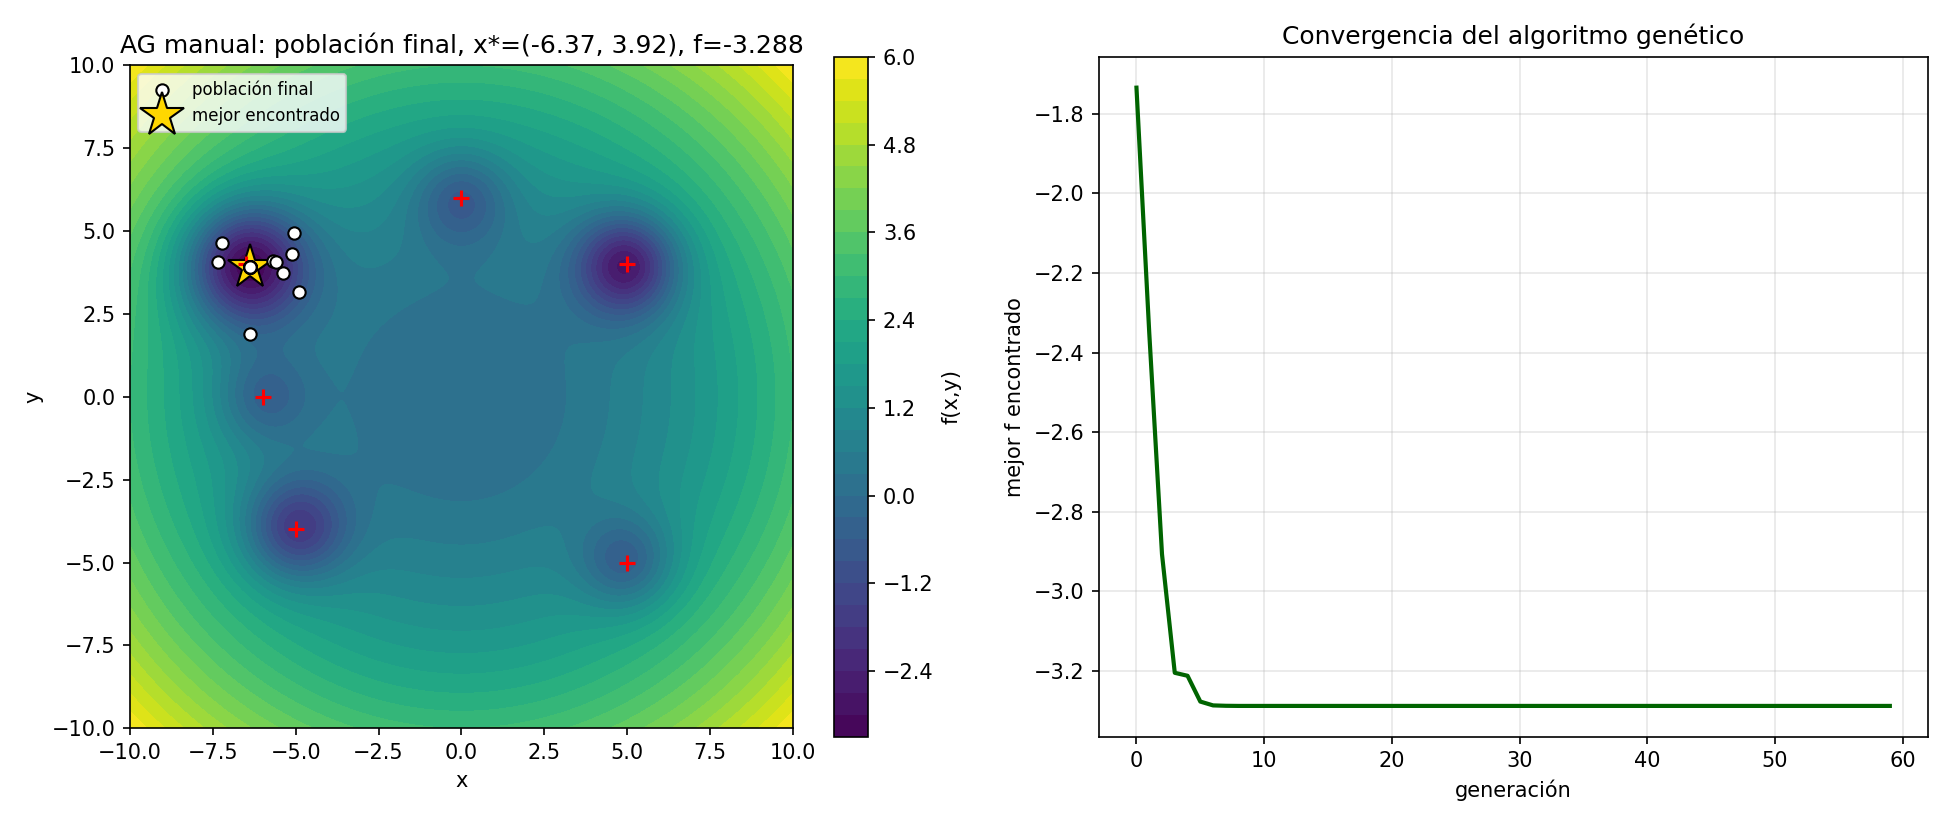
\includegraphics[width=0.95\textwidth,height=5.6cm,keepaspectratio]{fig05_algoritmo_genetico.png}
  \end{center}
  \footnotesize 30 individuos, 60 generaciones: converge al global en
  $\sim$10 generaciones y la población final se concentra alrededor del
  mejor pozo. $x^*=(-6.37,3.92)$, $f^*=-3.288$.
\end{frame}

\begin{frame}[fragile]{Algoritmos genéticos: manual vs.\ scipy}
\begin{lstlisting}
from scipy.optimize import differential_evolution

res = differential_evolution(
    lambda p: f(p[0], p[1]),
    bounds=[(-10,10),(-10,10)],
    popsize=15, maxiter=60, seed=0)
\end{lstlisting}
  \small \texttt{differential\_evolution} es también un algoritmo
  evolutivo poblacional (misma familia), pero con un operador de
  mutación distinto (diferencias vectoriales entre individuos, en vez
  de gaussiana) — típicamente más robusto y rápido para uso general.
  Ambos llegan a $f^*=-3.288$ (el global). Script:
  \texttt{scripts/05\_algoritmos\_geneticos.py}
\end{frame}

% ==================================================================
\section{Particle swarm optimization}
% ==================================================================

\begin{frame}{PSO: la idea (Kennedy \& Eberhart, 1995)}
  \begin{block}{Un enjambre que \emph{vuela} sobre el paisaje}
    Cada partícula $i$ tiene posición $\x_i$ y velocidad $\mathbf v_i$, y
    recuerda su mejor posición histórica $\mathbf p_i$
    (\emph{personal best}). El enjambre completo conoce la mejor
    posición global $\mathbf g$ (\emph{global best}).
  \end{block}
  \[
    \mathbf v_i \leftarrow \underbrace{w\,\mathbf v_i}_{\text{inercia}}
      + \underbrace{c_1 r_1(\mathbf p_i - \x_i)}_{\text{cognitivo}}
      + \underbrace{c_2 r_2(\mathbf g - \x_i)}_{\text{social}}
    \qquad
    \x_i \leftarrow \x_i + \mathbf v_i
  \]
  con $r_1,r_2\sim U(0,1)$ (aleatoriedad en \emph{cuánto} confiar en cada
  tendencia, no en si moverse o no).
  \begin{itemize}
    \item $w$ grande $\to$ más exploración; chico $\to$ converge más
      rápido.
    \item $c_1$: qué tanto confía la partícula en su \textbf{propia}
      experiencia.
    \item $c_2$: qué tanto confía en la experiencia del \textbf{grupo}.
  \end{itemize}
\end{frame}

\begin{frame}[fragile]{PSO: código manual (núcleo)}
\begin{lstlisting}
def pso_manual(n_particulas=25, n_iter=60, w=0.7, c1=1.5, c2=1.5, seed=0):
    x = rng.uniform(lo, hi, size=(n_particulas, 2))
    v = rng.uniform(-1, 1, size=(n_particulas, 2))
    p_best = x.copy();  f_p_best = f(x[:,0], x[:,1])
    g_best = p_best[np.argmin(f_p_best)].copy()
    for it in range(n_iter):
        r1, r2 = rng.random((n_particulas,2)), rng.random((n_particulas,2))
        v = w*v + c1*r1*(p_best - x) + c2*r2*(g_best - x)
        x = np.clip(x + v, lo, hi)
        f_x = f(x[:,0], x[:,1])
        mejora = f_x < f_p_best
        p_best[mejora], f_p_best[mejora] = x[mejora], f_x[mejora]
        ig = np.argmin(f_p_best)
        if f_p_best[ig] < f_g_best: g_best, f_g_best = p_best[ig].copy(), f_p_best[ig]
\end{lstlisting}
\end{frame}

\begin{frame}{PSO: ¿cómo arrancan \texttt{p\_best} y \texttt{g\_best}?}
  \begin{block}{\texttt{p\_best} inicial: la posición de nacimiento}
    Cada partícula solo conoce, al inicio, el punto aleatorio donde
    nació -- no hay nada más con qué comparar todavía. Por eso
    \texttt{p\_best = x.copy()}: su memoria personal arranca siendo,
    simplemente, su propio punto de partida.
  \end{block}
  \begin{block}{\texttt{g\_best} inicial: la mejor entre las $N$
    posiciones de nacimiento}
    Aquí sí hay una comparación real: se evalúa $f$ en las $N$
    posiciones iniciales y se toma la que dio el valor más bajo. No es
    al azar -- es una búsqueda directa del mínimo entre $N$ valores ya
    calculados.
  \end{block}
  Al momento cero cada partícula ``cree'' que su propio punto de
  partida es lo mejor que existe (es lo único que conoce), pero el
  enjambre ya sabe cuál de esas $N$ creencias individuales es,
  objetivamente, la mejor -- y eso le da una dirección común desde la
  primera iteración, en vez de volar sin rumbo.
\end{frame}

\begin{frame}{PSO: enjambre final y convergencia}
  \begin{center}
    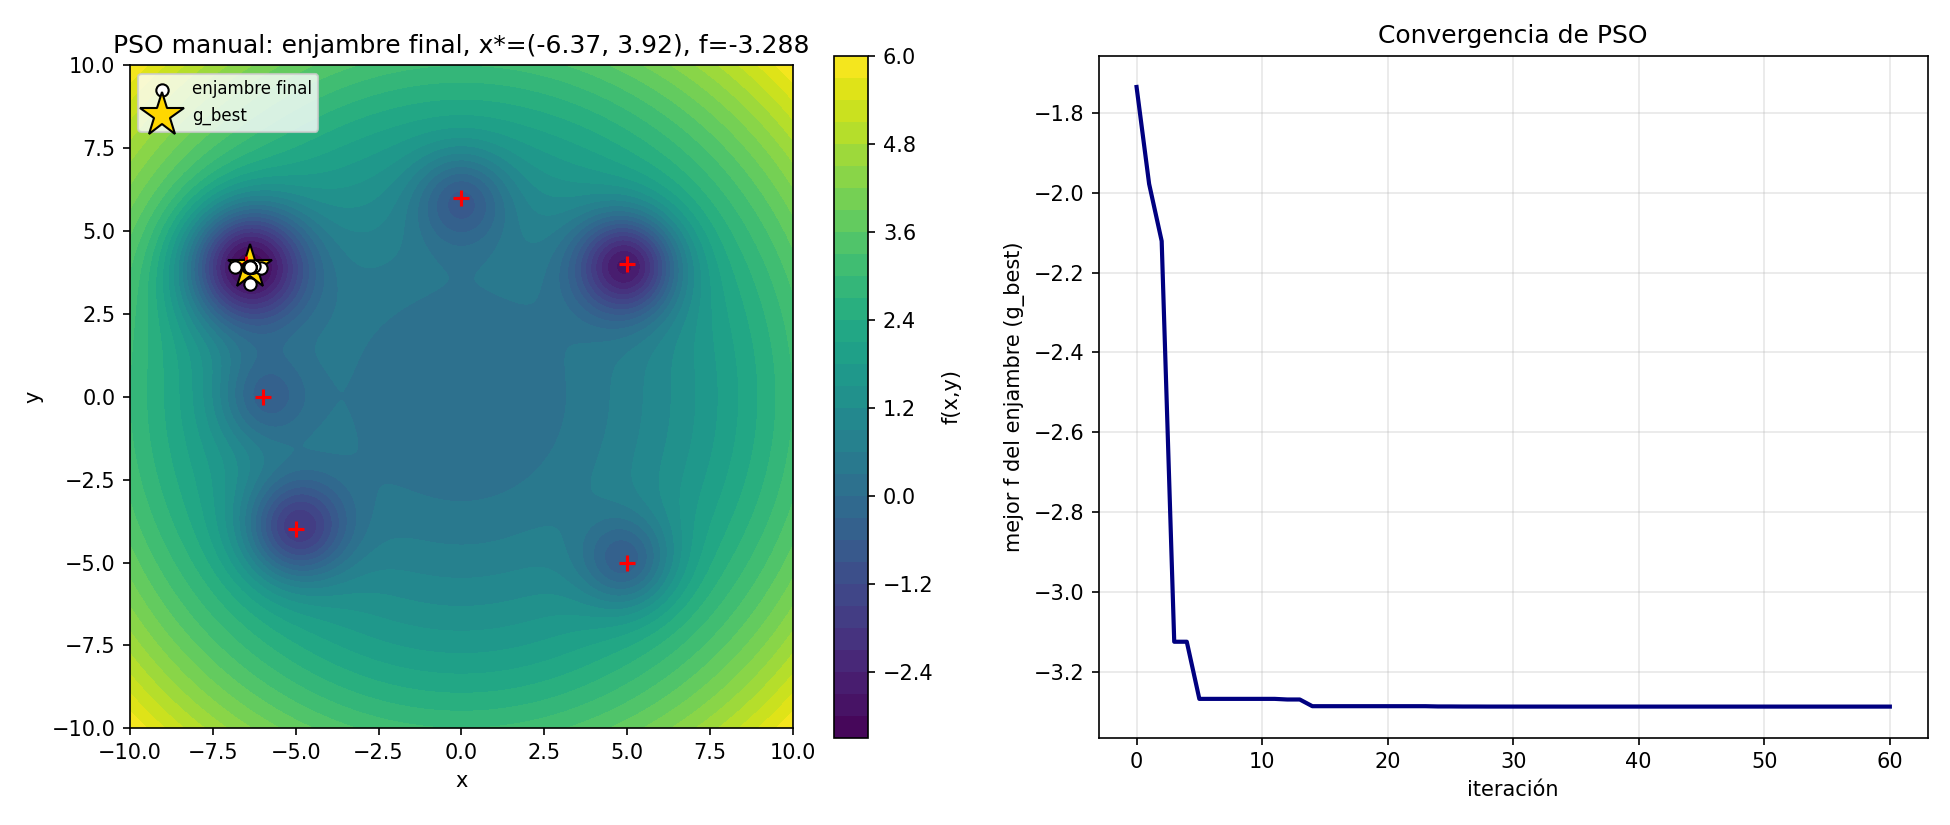
\includegraphics[width=0.95\textwidth,height=5.6cm,keepaspectratio]{fig06_particle_swarm.png}
  \end{center}
  \footnotesize 25 partículas, 60 iteraciones: el enjambre converge y se
  agrupa alrededor del mínimo global en $\sim$15 iteraciones —
  visiblemente más rápido que GA en este paisaje. $x^*=(-6.37,3.92)$,
  $f^*=-3.288$.
\end{frame}

\begin{frame}{PSO: ¿y la comparación con scipy?}
  \begin{alertblock}{Scipy no tiene PSO nativo}
    \texttt{scipy.optimize} no incluye particle swarm optimization. La
    familia evolutiva/poblacional más cercana disponible sigue siendo
    \texttt{differential\_evolution} (mismo espíritu: población,
    sin gradiente, sin garantías de optimalidad global, pero robusto en
    la práctica).
  \end{alertblock}
  \begin{itemize}
    \item Para PSO \emph{de verdad} en Python, la librería externa de
      referencia es \textbf{\texttt{pyswarms}} (no incluida en scipy).
    \item Vale la pena notarlo como ejemplo de que \textbf{no todos los
      métodos clásicos de optimización global tienen una función lista
      en scipy} — a veces hay que implementarlos, o buscar una librería
      especializada.
  \end{itemize}
  Script completo: \texttt{scripts/06\_particle\_swarm.py}
\end{frame}

% ==================================================================
\section{Síntesis}
% ==================================================================

\begin{frame}{Nueve métodos, un mismo paisaje}
  \tiny
  \begin{center}
  \begin{tabular}{lccccc}
    \toprule
    & \textbf{Grid search} & \textbf{Random walk} & \textbf{Nelder--Mead}
      & \textbf{Basin hopping} & \textbf{Sim.\ annealing} \\
    \midrule
    Tipo & exhaustivo & estocástico & local & metaheur.\ & metaheur.\ \\
    Población & -- & 1 punto & 1 simplex & 1 cadena & 1 cadena \\
    Escapa mínimos locales & sí (fuerza bruta) & no & no & sí & sí \\
    Costo & $O(N^d)$ & $O(\text{iter})$ & $O(\text{iter})$ &
      $O(\text{iter}\times\text{local})$ & $O(\text{iter})$ \\
    \bottomrule
  \end{tabular}
  \vspace{4pt}
  \begin{tabular}{lccc}
    \toprule
    & \textbf{Algoritmos genéticos} & \textbf{PSO} & \\
    \midrule
    Tipo & metaheur.\ poblacional & metaheur.\ poblacional & \\
    Población & $N$ individuos & $N$ partículas & \\
    Escapa mínimos locales & sí (diversidad) & sí (diversidad) & \\
    Costo & $O(\text{iter}\times N)$ & $O(\text{iter}\times N)$ & \\
    \bottomrule
  \end{tabular}
  \end{center}
  \normalsize
  \vspace{6pt}
  \small Los tres últimos (basin hopping, SA, GA/PSO) todos usan
  aleatoriedad \textbf{con criterio}: no exploran a ciegas como random
  walk puro, ni exhaustivamente como grid search.
\end{frame}

\begin{frame}{Lo que tienen en común}
  \begin{block}{El hilo conductor de las Clases 2 y 3}
    Todas las metaheurísticas de hoy resuelven el mismo problema:
    \textbf{cómo decidir cuándo aceptar una solución peor} para poder
    escapar de mínimos locales, sin degenerar en búsqueda puramente
    aleatoria.
    \begin{itemize}
      \item Basin hopping y SA: un parámetro de temperatura $T$
        (fijo o decreciente) controla esa probabilidad, vía Metrópolis.
      \item GA y PSO: la \textbf{diversidad de una población} cumple un
        papel similar — mientras algunos individuos convergen, otros
        siguen explorando.
    \end{itemize}
  \end{block}
  \begin{exampleblock}{Ninguno garantiza el óptimo global}
    Todos son heurísticos: mejoran mucho la probabilidad de encontrar el
    mínimo global frente a un método puramente local, pero
    \textbf{ninguno lo garantiza} en tiempo finito (salvo grid search,
    que sí lo garantiza pero a costo exponencial).
  \end{exampleblock}
\end{frame}

\begin{frame}{Un detalle que comparten los cuatro: ¿cuándo paran?}
  \begin{alertblock}{En los scripts de esta clase}
    Basin hopping, SA, GA y PSO se detienen aquí por
    \textbf{presupuesto fijo}: un número prefijado de iteraciones o
    generaciones (\texttt{n\_iter}, \texttt{n\_gen}), sin preguntar en
    ningún momento si ya conviene parar. Es el criterio más fácil de
    programar, pero también el menos eficiente.
  \end{alertblock}
  \begin{block}{Lo que se usa en la práctica}
    \begin{itemize}
      \item \textbf{Estancamiento}: parar si el mejor valor no mejora
        en las últimas $M$ iteraciones/generaciones seguidas.
      \item \textbf{Meta de calidad conocida}: parar al alcanzar un
        valor objetivo -- solo sirve si se conoce de antemano, como en
        un ejemplo de clase; en un problema real casi nunca se tiene.
      \item \textbf{Diversidad/dispersión}: parar si la población o el
        enjambre ya se agruparon mucho (poca varianza entre ellos).
      \item \textbf{Presupuesto de cómputo real}: tiempo de reloj o
        número de evaluaciones de $f$, útil cuando evaluar $f$ es caro
        (por ejemplo, si cada evaluación corre una simulación).
    \end{itemize}
  \end{block}
\end{frame}

% ==================================================================
\section{Roadmap del curso}
% ==================================================================

\begin{frame}{¿Qué sigue después de las Clases 1--3?}
  \begin{block}{Ya cubrimos}
    \begin{itemize}
      \item Clase 1: fundamentos (gradiente, Hessiana, convexidad,
        Lagrange/KKT).
      \item Clases 2--3: métodos de búsqueda, de lo determinista
        (bisección, grid search) a lo metaheurístico (basin hopping,
        SA, GA, PSO).
    \end{itemize}
  \end{block}
  \begin{alertblock}{Lo que falta}
    \begin{itemize}
      \item Método de \textbf{Newton} y métodos \textbf{cuasi-Newton}
        (BFGS, L-BFGS): usar curvatura (Hessiana o su aproximación) para
        converger mucho más rápido que el gradiente simple.
      \item \textbf{Programación lineal}: simplex, punto interior.
      \item \textbf{Programación no lineal con restricciones}: SQP,
        penalizaciones, barreras.
    \end{itemize}
  \end{alertblock}
\end{frame}

% ==================================================================
\section{Ejercicios propuestos}
% ==================================================================

\begin{frame}{Ejercicios para la próxima clase}
  \footnotesize
  \begin{enumerate}
    \item Modifique \texttt{scripts/01\_basin\_hopping.py} probando
      \texttt{step\_size} $\in\{2,5,10,15\}$ y $T\in\{0.3,1.5,5\}$.
      ¿Qué combinación encuentra el global con más frecuencia en 10
      corridas con semillas distintas?
    \item Implemente un esquema de enfriamiento \textbf{lineal}
      ($T_k=T_0(1-k/n_{\text{iter}})$) para simulated annealing y
      compárelo contra el geométrico del script
      \texttt{04\_simulated\_annealing.py}.
    \item En el algoritmo genético, quite el elitismo
      (\texttt{n\_elite=0}) y observe qué pasa con la curva de
      convergencia. ¿Por qué puede el mejor \texttt{f} \emph{empeorar}
      de una generación a otra sin elitismo?
    \item Modifique PSO para que $w$ decrezca linealmente de $0.9$ a
      $0.4$ durante las iteraciones (\emph{inertia weight damping}, muy
      usado en la práctica). ¿Mejora la convergencia?
    \item \textbf{Comparación final:} corra los 4 métodos de esta clase
      10 veces cada uno (semillas distintas) sobre el paisaje de 6
      pozos, y grafique un histograma de $f^*$ encontrado por cada
      método. ¿Cuál es más consistente?
    \item \textbf{Reflexión:} explique con sus palabras por qué basin
      hopping y GA/PSO pueden considerarse \emph{primos}: ambos mantienen
      múltiples candidatos (una cadena con reinicios vs.\ una
      población), aunque basin hopping los explore uno a la vez.
  \end{enumerate}
\end{frame}

% ==================================================================
\section{Referencias}
% ==================================================================

\begin{frame}{Referencias}
  \footnotesize
  \begin{itemize}
    \item D. Wales, J. Doye. \emph{Global Optimization by Basin-Hopping and
      the Lowest Energy Structures of Lennard-Jones Clusters}.
      J.\ Phys.\ Chem.\ A, 101(28), 1997.
    \item S. Kirkpatrick, C. Gelatt, M. Vecchi. \emph{Optimization by
      Simulated Annealing}. Science, 220(4598), 1983.
    \item J. Holland. \emph{Adaptation in Natural and Artificial
      Systems}. University of Michigan Press, 1975.
    \item D. Goldberg. \emph{Genetic Algorithms in Search, Optimization,
      and Machine Learning}. Addison-Wesley, 1989.
    \item J. Kennedy, R. Eberhart. \emph{Particle Swarm Optimization}.
      \emph{Proc.\ IEEE Int.\ Conf.\ on Neural Networks}, 1995.
    \item M. Kochenderfer, T. Wheeler. \emph{Algorithms for
      Optimization}. MIT Press, 2019. (Cap.\ 8--9: metaheurísticas
      poblacionales y basadas en temperatura, con código.)
    \item J. Nocedal, S. Wright. \emph{Numerical Optimization}, 2.\textsuperscript{a}
      ed. Springer, 2006.
    \item Documentación de \texttt{SciPy} (\texttt{scipy.optimize}):
      \url{https://scipy.org}.
    \item \texttt{pyswarms}: librería especializada de PSO en Python
      (no incluida en scipy): \url{https://pyswarms.readthedocs.io}.
  \end{itemize}
\end{frame}

\begin{frame}[standout]
  ¿Preguntas?
\end{frame}

\end{document}
